\chapter{Question 5 - Extended and Unscented Kalman Filter}
\assignment{
  \begin{enumerate}
    \item When is this estimation methods needed?
    \item What are the differences in theory and practice?
  \end{enumerate}
}

\assignment{1. When is this estimation methods needed?}
\section*{EKF}
The Extended Kalman Filter is used as an estimator for when the system dynamics is weak Non-linear (Almost linear).
\begin{itemize}
        \item Works for Sufficiently smooth systems.
        \item Stability not guaranteed.
        \item Convergence not guaranteed.
        \item Calculations of the Jacobian can be very difficult.
        \item We need to have a good estimate of the initial state $\hat{x}_0$
\end{itemize}

% \textbf{luenberger observer:} Linear system \\
% \textbf{Kalman filter:} Cases where the system can be linearised(once) nicely for the entire desired set \\
% \textbf{Extended Kalman filter:} The EKF is good for non-linear systems, where a big span is needed, but no one linearisation can cover the span nicely. \\

\section*{UKF}
The Unscented Kalman filter is used for strong Non-linear systems
% \begin{figure}[H]
%         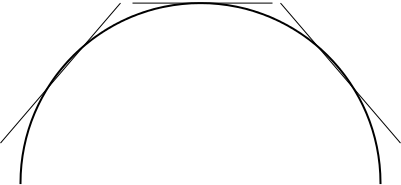
\includegraphics[width=5cm]{EKFsys.png}
% \end{figure}
% \textbf{Unscented Kalman filter:} The UKF is like the EKF needed for system which cannot be linearised for the entire span nicely. UKF is especially suited for system which is sporadic, and the local linearisation is insufficient.
% \begin{figure}[H]
%         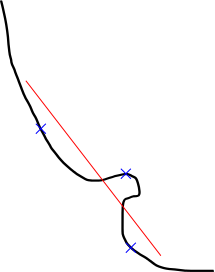
\includegraphics[width=5cm]{UKFsys.png}
% \end{figure}

\assignment{2. What are the differences in theory and practice?}
The EKF uses a nonlinear function to estimate the current output based on previous states and control signals. And uses a nonlinear function to predict the next states $\hat{x}_{k+1 \vert k}$
